\pdfminorversion=7
\documentclass[draft,linenumbers]{agujournal2025}
\usepackage{booktabs,amsmath,amssymb,microtype,url,graphicx,array}
\setlength{\emergencystretch}{3em}
\newcommand{\RSeeds}{20}
\newcommand{\RRecoveryAUC}{0.87}
\newcommand{\RWithinAUC}{0.81}
\newcommand{\RRetention}{94.8}
\newcommand{\RRisk}{0.8}
\newcommand{\RGroupExcess}{14.9}
\newcommand{\RTrendGain}{69.5}
\newcommand{\REuropeStations}{16}
\newcommand{\REuropeRequested}{16}
\newcommand{\REuropeErrors}{0}
\newcommand{\REuropeCases}{4474}
\newcommand{\REuropeAirCases}{458}
\newcommand{\REuropePowerMAE}{0.846}
\newcommand{\REuropeEraMAE}{0.777}
\newcommand{\RRecordDenominator}{96}
\newcommand{\RRecordStationYears}{35}
\newcommand{\RRecordStations}{20}
\newcommand{\RRecordHalfStations}{6}
\newcommand{\RPlanTwenty}{38.9}
\newcommand{\RPlanForty}{30.6}
\newcommand{\RPlanHundred}{19.2}
\newcommand{\RPlanTwoHundred}{13.4}

\newcommand{\WAStations}{42}
\newcommand{\WARepetitions}{3,320}
\newcommand{\WAOfflineCoverage}{94.0}
\newcommand{\WAForwardCoverage}{88.0}
\newcommand{\WABlockForwardCoverage}{89.0}
\newcommand{\WARetentionShare}{93.0}
\newcommand{\WADTwoMAE}{0.337}
\newcommand{\WAStochasticMAE}{0.336}
\newcommand{\WADTwoCoverage}{89.3}
\newcommand{\WAStochasticCoverage}{89.8}
\newcommand{\WADTwoCRPS}{0.246}
\newcommand{\WAStochasticCRPS}{0.245}
\newcommand{\WADTwoCRPSWins}{7}
\newcommand{\WADTwoTailWins}{0}
\newcommand{\WAWarmAdmitted}{32}
\newcommand{\WAWarmExcludedExceed}{2}
\newcommand{\WATaskForwardN}{39}
\newcommand{\WATaskForwardPercent}{4.8}
\newcommand{\WADonorBase}{0.079}
\newcommand{\WADonorStress}{0.116}
\newcommand{\WAHeatBase}{0.035}
\newcommand{\WAHeatStress}{0.058}
\newcommand{\WASelectedRMSE}{0.202}
\newcommand{\WASelectedBaseRMSE}{0.173}
\newcommand{\WASelectedCoverage}{99.8}
\newcommand{\WASelectedWidth}{3.26}
\newcommand{\WAQualityUnassessed}{185}
\newcommand{\WAQualityStrictRMSE}{0.040}
\newcommand{\WAAdditionalStations}{3}
\newcommand{\WAAdditionalYears}{9}

\begin{document}
\journalname{Water Resources Research}
\title{Incomplete river-temperature years: separating recovery, screening and trend inference}
\authors{[Author names]\affil{1}}
\affiliation{1}{[Affiliations]}
\authoraddr{[Corresponding author and email]}
\authorrunninghead{Anonymous}\titlerunninghead{Incomplete river-temperature years}
\keypoints
{Observed windows can disprove a complete-year-only heat record, but most witnesses pass a 90 percent warm-season rule}
{Distribution regression and calibrated stochastic reconstruction have similar annual accuracy in difficult gaps}
{Retaining years improves the evaluated finite-record trends; forward interval coverage and useful release remain limited}
\maketitle\par
\begin{abstract}
Incomplete river-temperature years can contain information about sustained heat, but the evidence needed to recover an annual value, release it, or infer a trend differs. At \RRecordStations{} of \RRecordDenominator{} long-record stations, fully observed 30-day windows in \RRecordStationYears{} incomplete years exceed every complete-year heat maximum. Of these witnesses, \WAWarmAdmitted{} pass a station-specific 90\% warm-season rule, so the observation-only result mainly challenges strict annual completeness. Across twenty source repetitions, annual distribution regression (D2) and equally calibrated stochastic reconstruction have similar errors on difficult gaps. We jointly degrade multiyear archives at \WAStations{} stations before local refitting and compare retention and estimator effects on the same finite-record slopes. Bounded annual distributions use a stated tail extrapolation and identical marginals across three joint-rank constructions. For controlled gaps, nominal 95\% D2 trend intervals cover \WAOfflineCoverage\% offline and \WAForwardCoverage\% in retrospective forward evaluation. Task-level calibration is available for \WATaskForwardPercent\% of forward controlled-gap cases under empirical support checks, with no population coverage guarantee. A three-output rule retains bounds or withholds values, but its individual classifier score does not certify group risk. Exploratory Canadian comparisons use published daily means or reported-hour records with unresolved quality or time basis; independent strict-reference validation remains open. These findings support preserving observed heat information while restricting claims about numerical recovery, transfer and trend uncertainty.
\begin{plainlanguagesummary}
Gaps in a river's water-temperature record do not necessarily erase information about a hot year. If thirty consecutive observed days are already warmer than the record among fully observed years, the complete-year-only record is incomplete. Most such examples in our archive would also be retained by a less restrictive warm-season rule. We compared several ways to estimate missing values and then tested what they imply for a trend across many years. A calibrated classical reconstruction was about as accurate as a more elaborate annual model. Trend intervals were less reliable when applied to later years, and screening rules did not provide a general safety guarantee. The analysis distinguishes observed facts, estimated values and cases where the evidence is insufficient.
\end{plainlanguagesummary}
\end{abstract}

\section{Introduction}
Stream-temperature records support studies of thermal habitat, climate change and water management \cite{caissie2006,michel2020,vanhamel2024}. The annual maximum of a 30-day mean summarizes sustained heat and is related to the thermal peak used in river-network studies \cite{beaufort2022}. A monitoring gap can affect this statistic very differently depending on its timing, the observations remaining in the year and the information available from other years or stations.

Prior work has already shown that partial stream-temperature records can support some annual analyses. \citeA{johnson2021} evaluated missing intervals and imputation for annual mean, phase and amplitude, finding limitations that varied among rivers. \citeA{beaufort2022} used summer observations and climate correction for a multiyear thermal-peak metric. Neither should be interpreted as requiring every calendar year to be complete. Our question is narrower: what do incomplete daily records support about an annual sustained-heat maximum, numerical publication, and a finite-record trend? We compare strict completeness with a station-specific warm-season rule and distinguish a mathematical observation bound from model-based estimation.

Regression record augmentation and maintenance-of-variance methods have a long hydrological history \cite{matalas1964,hirsch1982,vogel1985}. A point prediction, a predictive distribution and a decision to release a value have different targets. Distributional imputation should be assessed for the downstream quantity rather than only for daily squared error \cite{naf2023,gneiting2007}. Here we compare a daily plug-in, simple corrections, calibrated stochastic reconstruction and annual distribution regression. We then jointly hide portions of a station's multiyear record before local refitting and evaluate whether retaining years changes the slope of that finite record. Finally, we examine whether the annual distributions support trend uncertainty and whether visible information can identify cases that should not receive a numerical estimate.

The hypotheses are deliberately conditional: target-oriented recovery can improve on a daily plug-in without necessarily beating a calibrated stochastic comparator; retaining years can improve a finite-record slope under a specified degradation mechanism; and annual and trend uncertainty require separate evaluation. The evidence map in Table~\ref{tab:evidence-map} identifies the comparisons and limits.
\begin{table}[t]\centering
\fontsize{8}{10}\selectfont
\renewcommand{\arraystretch}{1.08}
\newcolumntype{L}[1]{>{\raggedright\arraybackslash}p{#1}}
\setlength{\tabcolsep}{4pt}
\hyphenpenalty=10000\exhyphenpenalty=10000
\caption{Evidence map. Each claim is paired with the comparison and metric used here and with the boundary that limits it. The table indexes the results; it is not an additional test.}\label{tab:evidence-map}
\begin{tabular}{L{0.18\textwidth}L{0.26\textwidth}L{0.20\textwidth}L{0.25\textwidth}}
\toprule
Claim & Primary comparison & Metric & Boundary \\
\midrule
Observed windows can overturn a complete-only record & Complete-year H30 vs.\ fully observed 30-day window $L$ & Count of $L$ above the complete-year maximum & Reported measurements only; not the unique warmest year \\
Target recovery beats a daily plug-in & D2 vs.\ plug-in, functional debiasing and calibrated stochastic regression & H30 MAE, CRPS and 90\% coverage & No unique gain over calibrated stochastic regression \\
Retaining years improves finite-record trends & Warm-season rule vs.\ all supported years at the same estimator & Trend RMSE; symmetric retention and estimator shares & Shares are setting-specific, not a universal percentage \\
Annual and trend uncertainties need distinct evaluation & Bounded normal-tail vs.\ constant-tail marginals; three rank couplings & Coverage, width, interval score and availability & Tail, annual and dependence errors are not uniquely separated \\
Numerical release has a risk--retention trade-off & Fixed score cap vs.\ three-output rule & Selected risk, retention and group excess & A raw individual score is not a group-risk guarantee \\
Visible diagnostics do not restore extrapolation safety & Clean vs.\ hot-year, future-year and air-exposure stress & Selected risk, coverage and retention & Synthetic stress severity; not an archive prevalence \\
\bottomrule
\end{tabular}
\end{table}


\section{Data and study design}
The source archive contains previously assembled European and US daily observations: 581 physical stations, 185 connected-record groups, 27 regions and 6,170 unique complete station-years. NASA POWER daily air temperature is the common meteorological input \cite{nasapower2026}. Artificial controlled gaps of 30, 60 or 90 days are crossed with overlap with a training-period climatological peak window; empirical incomplete calendars provide a separate family. Each of twenty source repetitions redraws masks and group-role composition. In the leave-one-year-out source comparison, fitting, interval calibration, score learning and rule calibration use disjoint connected groups outside each held region. These repetitions describe variability within the available archive, not twenty independent climates. Figure~\ref{fig:architecture} separates the observation-only, single-year and whole-archive evidence.

We use complete daily station-years as reference outcomes for artificial masking. Water observations hidden by a mask never enter the local fit for that case. Features available when a value is evaluated include the visible gap geometry, a training-period climatological peak, local water history, air conditions and available neighboring stations. The true peak location and hidden water values are evaluation quantities. Observation quality is inherited from the assembled source records; a reported value is not assumed to be error-free physical truth. An observed lower bound is valid for the reported series if its thirty measurements are comparable and valid.

The annual target is
\begin{equation}
 H30_y=\max_{j}\frac{1}{30}\sum_{d=j}^{j+29}Y_{yd}.
\end{equation}
For an incomplete year, the largest fully observed 30-day mean $L_y$ satisfies $H30_y\ge L_y$ for the same reported series. For 1981--2025 we select stations with at least fifteen complete reference years and compare every incomplete-year bound with the largest complete-year H30. We also evaluate whether those same witnesses pass a 95\% annual-coverage rule and a 90\% station-specific warm-season rule. The five consecutive warm months are obtained from the station's climatology after excluding the evaluated year. These are explicit study comparators; the seven-week missing-period result of \citeA{johnson2021} concerns annual signal parameters, not a validated H30 record rule.
\begin{figure}[t]\centering
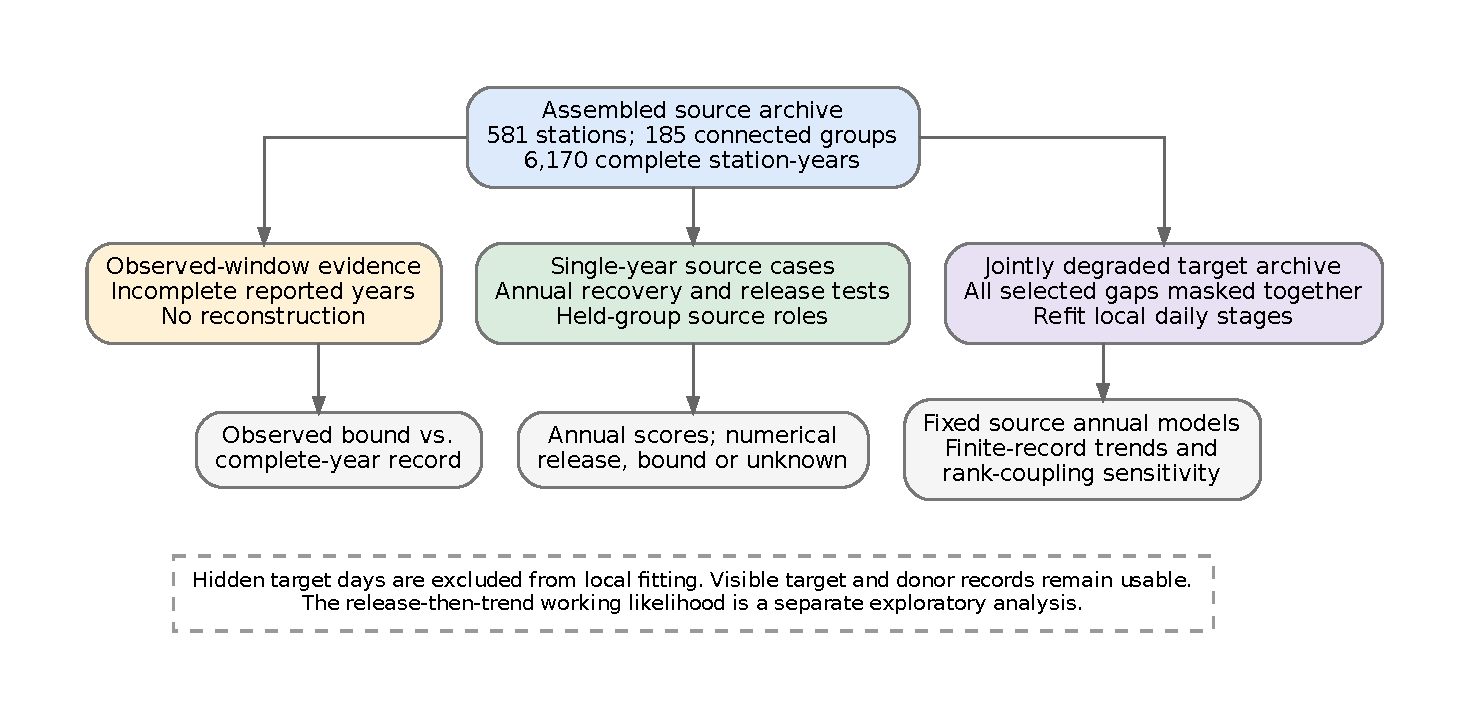
\includegraphics[width=\textwidth]{figures/architecture/fig1_evidence_actual.pdf}
\caption{Evidence architecture. Observation-only witnesses, single-year source evaluations and jointly degraded target archives address distinct questions. Hidden target days are excluded from local fitting; unmasked target and donor records remain available. Annual source models are fitted separately and held fixed during each archive reanalysis. Release followed by the working-likelihood trend is a separate exploratory analysis.}\label{fig:architecture}
\end{figure}

\newcommand{\SWStations}{95}
\newcommand{\SWGroups}{33}
\newcommand{\SWComplete}{2,122}
\newcommand{\SWAbove}{779}
\newcommand{\SWAboveHalf}{304}
\newcommand{\SWMean}{0.255}
\newcommand{\SWExclYears}{2,086}
\newcommand{\SWExclAbove}{749}
\newcommand{\SWExclMean}{0.197}
\newcommand{\SWWitness}{9}
\newcommand{\SWRuleYears}{2,656}
\newcommand{\SWWarmRejected}{66}
\newcommand{\SWWarmBounds}{50}
\newcommand{\SWAnnualRejected}{106}
\newcommand{\SWAnnualBounds}{90}

\newcommand{\PWYears}{2,656}
\newcommand{\PWChange}{1}
\newcommand{\PWMinimumDays}{1}
\newcommand{\PWUnknown}{127}
\newcommand{\PWUnknownBounds}{122}
\newcommand{\PWWitnessAccepted}{27}
\newcommand{\PWWitnessRejected}{2}
\newcommand{\PWWitnessUnknown}{6}
\newcommand{\PWWitnessPrior}{2}


\section{Methods}
\subsection{Annual recovery and decision to release}
The daily plug-in computes H30 after a selected daily reconstruction. Functional debiasing corrects its annual value, whereas D2 learns annual-error quantiles using visible features and simulated trajectories. A stochastic regression comparator generates conditional residual bridges and calculates H30 for each realization. D2 and the stochastic comparator have the same source interval-calibration roles and bootstrap multiplicities. Point estimates are medians; MAE, CRPS, 90\% interval coverage and interval score are reported on available cases, with paired comparisons on common cases.

In the twenty historical source fits, we apply the same observed-window support projection to both methods after their original calibration. The seven stored quantiles do not determine their outer tails; for comparable CRPS integration we extend the tails using adjacent normal-quantile spacings and enforce $L_y$ when available. The original model weights and calibration offsets remain fixed in this source re-analysis. In the whole-archive study described below, offsets for both methods are instead re-estimated on their original independent calibration roles after projection. Neither approach makes the assumed tail shape a verified full distribution.

The conditional-mean mechanism is useful but limited. For observed information $X$ and 30-day averaging vectors $w_j$, convexity gives
\[
 \max_j w_j^\top E(Y\mid X)\le E\{\max_j w_j^\top Y\mid X\}.
\]
It concerns the true conditional mean and conditional expectation; an approximate learner need not underestimate every individual year. Calibration, local adaptation, model bias and the chosen point summary remain empirical questions.

We evaluate a rule that reports an estimated value, an observed lower bound or an unknown state. Numerical release requires an available D2, at least four complete historical years, visible features within source-derived limits and a raw individual classifier score no greater than 0.10. The score was trained for the original unprojected D2 and is not a calibrated group-risk certificate for the projected value. A seven-day close match between visible water and air temperature is tested for the imposed exact-air-substitution scenario; that detector is not evaluated for other stresses. No observed bound is released when this quality flag is raised. The primary factorial trend comparison is separate. A second exploratory analysis passes released values and bounds into a Gaussian working likelihood, treating released numerical estimates as exact and each bound $L$ as a right-censored response with contribution $P(H30\ge L)$. Unknown cases remain in availability denominators. The resulting regression interval includes working-model variability and is not a task-calibrated missingness-only interval.

\subsection{Whole-archive degradation and task-level uncertainty}
The whole-archive benchmark jointly masks selected gaps in several years of a target station before fitting its daily models, climatology or residual histories. Unmasked target observations and neighboring physical stations remain available in this experiment. The benchmark contains 42 stations with at least twenty complete reference years in seven regions. One Finnish record ends in 1994, leaving 41 stations for forward evaluation. Twenty paired mask repetitions use both empirical calendars and controlled 30--90-day gaps; after seven observed burn-in years, each reference year is degraded with probability 0.35. These 3,320 archive experiments do not reuse any masked target day when fitting another year. The complete reference, including those hidden days, is used for scoring; its unmasked values can also enter local fitting. The archived single-year plug-in is retained as an optimistic-information paired comparator on identical masks.

Offline daily fits use the remaining visible history. Forward annual models and interval offsets use source observations before 2010 and exclude the evaluated test stations and their connected groups. The original partitioned role assignment can retain other training-only groups in the same named region: this occurs in the HUC17 estimator and in NVE interval calibration. Accordingly this forward experiment is held-test-group, not uniformly held-region, and is applied to 2010 onward. Forward local daily fitting and dependence estimation also exclude water observations from 2010 onward. These are current-vintage retrospective forward experiments, not a historical real-time field trial. Annual regression weights remain source-only and use source-fit seed zero throughout. Source observations do not change across archive masks, so those fits are reused; every local stage that uses the degraded target archive is refitted. Twenty archive masks are not twenty new global model fits.

On each degraded archive, the retention set (90\% warm-season rule or all supported years) is crossed with the annual estimator (daily plug-in, equally calibrated stochastic regression or D2). Every slope is scored against the same complete-record slope. For the four MSE cells $A$ (rule/plug-in), $B$ (all/plug-in), $C$ (rule/alternative) and $D$ (all/alternative), the symmetric retention contribution is $\{(A-B)+(C-D)\}/2$, and the estimator contribution is $\{(A-C)+(B-D)\}/2$. They sum to $A-D$; the interaction is $(A-B)-(C-D)$. Complete paired cells, rather than different available subsets, determine each decomposition.

We refit both methods' annual quantile offsets on their original disjoint source calibration groups after imposing the observed-window lower bound. Both distributions and their samples respect the bound when one is available. Seven stored quantiles identify only the central 90\% of the distribution. We extrapolate both outer tails using the adjacent normal-quantile spacing and project samples onto the bound; the endpoint-constant alternative is retained on paired cases. The normal extrapolation is an assumption, not a validated tail law. We use 256 stratified samples per year and compare independent ranks, auxiliary shared year-bootstrap regression states, and three-year residual blocks on exactly the same annual marginals. Shared states come from a small harmonic/air Ridge model, not the D2 tree posterior or the selected donor model. These couplings are dependence sensitivities, not posterior samples or coverage theorems.

The task-level comparator calibrates absolute slope error divided by an independent-draw interval half-width. Every source connected group receives equal total weight in the empirical 95th percentile. Calibration uses only unused rule-calibration groups, re-predicted with the held-region model; forward errors end before 2010. We withhold the calibration when fewer than three nondegenerate source groups remain, the calibration factor is effectively zero, or the target half-width lies outside the source 1st--99th percentile range. These thresholds are empirical support checks rather than a finite-sample guarantee. Source support, availability and matched-case width, coverage and interval score are reported. All uncertainty scores target the finite complete-record slope, not climate-trend uncertainty.


Two small stress studies select one long-record station per region and five mask repetitions. One applies the target's exact masks simultaneously to all observed donor stations; the other changes annual missingness probabilities to 0.90 or 0.18 according to whether the year's air H30 exceeds the first-seven-year 80th percentile. The latter changes the realized masks and missing-year count as well as the heat association. A station with insufficient air data is unavailable; neither study constitutes a new climatic replication.

\section{Results}
\subsection{What the observations establish}
\begin{figure}[t]\centering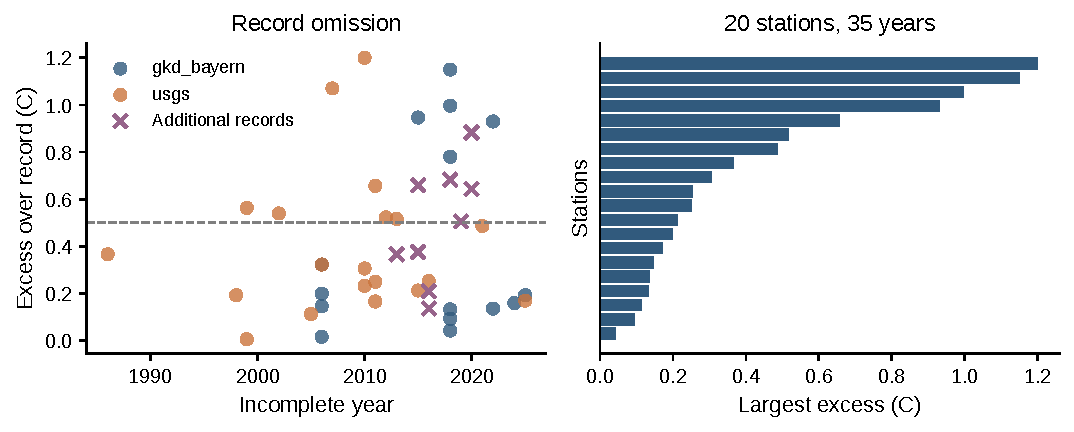
\includegraphics[width=\textwidth]{figures/simple_research/01_observed_records.pdf}\caption{Fully observed thirty-day windows in incomplete years exceed complete-only station records. Crosses on the left are additional approved-record witnesses with sparse one-to-three-year complete reference support; they are not included in the original long-record denominator or the source-station bars on the right. The evidence concerns reported measurements and requires no reconstruction.}\label{fig:observed-records}\end{figure}

At \RRecordStations{} of \RRecordDenominator{} eligible stations, \RRecordStationYears{} incomplete years contain an observed window above the maximum complete-year H30 (Figure~\ref{fig:observed-records}). Six stations have a witness exceeding the complete-year record by more than 0.5$^{\circ}$C. Another incomplete year could still be warmer, and measurement error or a changed sensor location can affect physical interpretation.

The practical consequence depends on the rule. Of the 35 witnesses, \WAWarmAdmitted{} pass the station-specific 90\% warm-season criterion and 31 pass 95\% annual coverage. Among those rejected by the warm-season criterion, \WAWarmExcludedExceed{} exceed the largest \emph{observed window} among rule-accepted years. A rule-accepted incomplete year may itself have an unobserved higher H30, so that comparison concerns reported windows rather than a proven full-record ordering. The evidence therefore establishes a cost of strict complete-year selection; it does not attribute all 35 omissions to the more permissive rule.

In a post-hoc seasonal-window diagnostic on the \SWStations{}-station subset with documented candidate reuse paths, \SWAbove{} of \SWComplete{} complete station-years have full-year H30 above the maximum 30-day mean entirely within July--August by more than $5\times10^{-6}$ $^{\circ}$C; \SWAboveHalf{} exceed it by more than 0.5 $^{\circ}$C. This reports differences in the assembled series, not sensor error. Among \SWRuleYears{} eligible station-years, the station-specific 90\% warm-season rule rejects \SWWarmRejected{}, of which \SWWarmBounds{} still contain a fully observed 30-day window. A bound is not an exact H30 or a demonstrated trend improvement. This comparison does not reproduce the multiyear climate correction of \citeA{beaufort2022}, whose study excluded strongly human-influenced sites. Two sites producing the largest individual differences are among the dam-affected locations studied by \citeA{rounds2010}; removing them post hoc leaves \SWExclAbove{} of \SWExclYears{} complete years with a difference above the numerical tolerance. Those earlier dam findings do not establish the cause of every difference here (Supporting Information).

The original warm-season climatology can use years later than the evaluated year. A retrospective past-only sensitivity changes \PWChange{} screening decision when any earlier observation is permitted, but this can mean as little as \PWMinimumDays{} prior day of data. Requiring four earlier complete years for incomplete-year screening leaves \PWUnknown{} of \PWYears{} station-years unknown; \PWUnknownBounds{} of those still have an observed 30-day bound. Of the 35 selected witnesses, \PWWitnessAccepted{} are accepted, \PWWitnessRejected{} rejected and \PWWitnessUnknown{} unknown. The station cohort and current data vintage are retrospective, so this is not an as-of-vintage prospective validation (Supporting Information).

\subsection{Additional observation-only corroboration}
We obtained approved daily-mean USGS temperature records at ten additional metadata-selected stream stations. None was a source-model target. Seven candidates lie in HUC2 regions 13 or 20, absent from the source station regions; three are additional station checks within already represented HUC2 regions. The candidates and all qualification failures are retained. This unregistered intake was not a random sample or a blinded confirmation, and the reference histories are shorter and sparser than the original long-record panel.

The unchanged four-complete-year reconstruction criterion yields zero eligible numerical-recovery references. The observation-only claim needs a different comparison: an incomplete year can contradict the maximum of the complete-year record whenever at least one approved-complete reference year exists. We retain every approved finite reference value, including reference years that an extra heuristic-QC filter might remove. Candidate windows must contain thirty consecutive approved, nonestimated daily values after source QC, and the incomplete year must have an actual absent, null, contradictory or unapproved provider day. Heuristic censoring alone cannot create a witness.

There are four stations with a nonempty approved-complete reference, each with only one to three reference years. At \WAAdditionalStations{} of these stations, \WAAdditionalYears{} incomplete station-years contain verified windows exceeding every approved-complete H30 in the analyzed record (Figure~\ref{fig:observed-records}; supporting information). For example, the Rio Mora 2020 window exceeds the complete-only record by approximately 0.883$^{\circ}$C, and a Pecos River 2020 window by 0.643$^{\circ}$C. These facts corroborate record omission without fitting any imputer. They do not estimate an omission incidence, verify a unique warmest year, establish external reconstruction accuracy, or validate trend or risk guarantees. Every witness includes the thirty original approved values; agency reporting and measurement validity remain assumptions.


\subsection{Annual point and distribution comparisons}
On controlled gaps overlapping at least half the training climatological peak, the median source-repetition H30 MAE is approximately 0.428$^{\circ}$C for the daily plug-in, 0.355 for functional debiasing, \WADTwoMAE{} for D2 and \WAStochasticMAE{} for calibrated stochastic regression (Figure~\ref{fig:estimators}). Median 90\% interval coverage is \WADTwoCoverage\% and \WAStochasticCoverage\%, respectively, with CRPS \WADTwoCRPS{} and \WAStochasticCRPS{}. On common cases D2 improves CRPS in \WADTwoCRPSWins{} of twenty repetitions and upper-tail CRPS in \WADTwoTailWins{}; equality of the methods is not established. Both distributions use the same support projection and tail approximation in this comparison; method-specific availability and paired counts are reported in Supporting Information Table S1. The practical evidence is a gain over the simple plug-in, not a demonstrated universal need for D2.

\newcommand{\UCCommon}{818}
\newcommand{\UCAll}{820}
\newcommand{\UCStations}{41}
\newcommand{\UCGroups}{17}
\newcommand{\UCAnnual}{90.1}
\newcommand{\UCAnnualEqual}{89.6}
\newcommand{\UCTailConstant}{83.0}
\newcommand{\UCTailNormal}{88.8}
\newcommand{\UCTailWidthConstant}{0.380}
\newcommand{\UCTailWidthNormal}{0.451}
\newcommand{\UCTailScoreConstant}{0.987}
\newcommand{\UCTailScoreNormal}{0.860}
\newcommand{\UCIndependent}{88.0}
\newcommand{\UCShared}{87.9}
\newcommand{\UCBlocks}{89.0}
\newcommand{\UCIndependentScore}{0.868}
\newcommand{\UCSharedScore}{0.854}
\newcommand{\UCBlocksScore}{0.830}

\newcommand{\SPCalendarCommon}{3,674}
\newcommand{\SPCalendarDTwoZero}{1,476}
\newcommand{\SPCalendarDTwoPercent}{40.2}
\newcommand{\SPCalendarClassicZero}{2,977}
\newcommand{\SPCalendarClassicPercent}{81.0}
\newcommand{\SPCalendarDTwoMiss}{0}
\newcommand{\SPCalendarClassicMiss}{0}
\newcommand{\SPCrossCommon}{3,683}
\newcommand{\SPCrossDTwoZero}{323}
\newcommand{\SPCrossClassicZero}{1,091}
\newcommand{\SPCrossClassicMiss}{3}
\newcommand{\SPCrossDTwoMedian}{1,186}
\newcommand{\SPCrossDTwoMedianAbove}{64}
\newcommand{\SPCrossClassicMedian}{1,375}
\newcommand{\SPCrossClassicMedianAbove}{61}
\newcommand{\SPCrossClassicMissStations}{2}
\newcommand{\SPCrossClassicMaxMiss}{0.143}
\newcommand{\SPCalendarDTwoCreatedLast}{380}
\newcommand{\SPCalendarDTwoBeforeLast}{1,096}
\newcommand{\SPCalendarClassicCreatedLast}{0}
\newcommand{\SPCalendarClassicRawZero}{3,090}

\newcommand{\PVCalendarAll}{3,674}
\newcommand{\PVCalendarVisible}{3,125}
\newcommand{\PVCalendarHidden}{549}
\newcommand{\PVCalendarDTwoCoverage}{88.3}
\newcommand{\PVCalendarClassicCoverage}{87.8}
\newcommand{\PVCrossAll}{3,683}
\newcommand{\PVCrossHidden}{2,146}
\newcommand{\PVCrossDTwoCoverage}{83.2}
\newcommand{\PVCrossClassicCoverage}{81.6}
\newcommand{\PVCrossDTwoCILow}{72.6}
\newcommand{\PVCrossDTwoCIHigh}{93.0}
\newcommand{\PVCrossClassicCILow}{72.2}
\newcommand{\PVCrossClassicCIHigh}{91.7}

\newcommand{\AEFwdCommon}{3,683}
\newcommand{\AEFwdSupported}{92}
\newcommand{\AEFwdPct}{2.5}
\newcommand{\AEFwdStations}{1}
\newcommand{\AEFwdDTwoBefore}{100.0}
\newcommand{\AEFwdDTwoAfter}{100.0}
\newcommand{\AEFwdClassicBefore}{100.0}
\newcommand{\AEFwdClassicAfter}{100.0}
\newcommand{\AEFwdDTwoWidthBefore}{0.532}
\newcommand{\AEFwdDTwoWidthAfter}{0.543}
\newcommand{\AEFwdClassicWidthBefore}{0.555}
\newcommand{\AEFwdClassicWidthAfter}{0.567}
\newcommand{\AEMaxSourceGroups}{4}

\newcommand{\NSExpCases}{144}
\newcommand{\NSExpStations}{2}
\newcommand{\NSExpYears}{8}
\newcommand{\NSExpDTwoMAE}{0.311}
\newcommand{\NSExpClassicMAE}{0.313}
\newcommand{\NSExpDTwoCover}{88.2}
\newcommand{\NSExpClassicCover}{93.1}
\newcommand{\NSExpDTwoWidth}{1.000}
\newcommand{\NSExpClassicWidth}{1.281}
\newcommand{\NSExpDTwoScore}{1.572}
\newcommand{\NSExpClassicScore}{1.706}

\newcommand{\NSClockCases}{144}
\newcommand{\NSClockHMax}{0.0023}
\newcommand{\NSClockDTwoMax}{0.094}
\newcommand{\NSClockDTwoMinus}{0.310}
\newcommand{\NSClockDTwoZero}{0.311}
\newcommand{\NSClockDTwoPlus}{0.315}
\newcommand{\NSClockClassicMinus}{0.313}
\newcommand{\NSClockClassicZero}{0.313}
\newcommand{\NSClockClassicPlus}{0.313}

\newcommand{\RHModels}{98}
\newcommand{\RHRoleRows}{392}
\newcommand{\RHHucGroups}{1}
\newcommand{\RHHucStations}{1}
\newcommand{\RHHucCases}{140}
\newcommand{\RHHucWeighted}{280}
\newcommand{\RHNveGroups}{2}
\newcommand{\RHNveStations}{3}
\newcommand{\RHNveCases}{431}
\newcommand{\RHArchiveCases}{120}
\newcommand{\RHArchiveStations}{3}
\newcommand{\RHFutureCases}{6,198}

\newcommand{\AURefYears}{80}
\newcommand{\AURefStations}{52}
\newcommand{\AUFirstCases}{30,728}
\newcommand{\AUFirstMatch}{80}
\newcommand{\AUFirstEvaluable}{79}
\newcommand{\AUFormerTest}{10}
\newcommand{\AUFormerTestEvaluable}{10}
\newcommand{\AUHotOverlap}{74}
\newcommand{\AUHotEvaluable}{73}

\newcommand{\RightsModelCombinations}{13}
\newcommand{\RightsEstimatorLUBW}{13}
\newcommand{\RightsCalibrationLUBW}{6}

\newcommand{\OpenSourcePairs}{738}
\newcommand{\OpenSourceGroups}{17}
\newcommand{\OpenSourceOldDTwo}{0.16381}
\newcommand{\OpenSourceOldClassic}{0.14658}
\newcommand{\OpenSourceNewDTwo}{0.15806}
\newcommand{\OpenSourceNewClassic}{0.15600}
\newcommand{\OpenSourceFactorCases}{807}
\newcommand{\OpenSourceOldRetention}{93.9}
\newcommand{\OpenSourceNewRetention}{93.7}
\newcommand{\OpenSourceCoverageCases}{820}
\newcommand{\OpenSourceOldCoverage}{88.0}
\newcommand{\OpenSourceNewCoverage}{87.6}

\newcommand{\OpenAnnualCases}{2146}
\newcommand{\OpenAnnualStations}{41}
\newcommand{\OpenAnnualGroups}{17}
\newcommand{\OpenAnnualDTwoOld}{83.2}
\newcommand{\OpenAnnualDTwoNew}{81.9}
\newcommand{\OpenAnnualClassicOld}{81.6}
\newcommand{\OpenAnnualClassicNew}{78.2}
\newcommand{\OpenAnnualDTwoWidthOld}{1.299}
\newcommand{\OpenAnnualDTwoWidthNew}{1.161}
\newcommand{\OpenAnnualClassicWidthOld}{1.121}
\newcommand{\OpenAnnualClassicWidthNew}{1.078}
\newcommand{\OpenAnnualClassicDelta}{-3.4}
\newcommand{\OpenAnnualClassicDropFoen}{+0.3}
\newcommand{\OpenAnnualClassicDropBayern}{-8.9}

\newcommand{\SYAllEligible}{3683}
\newcommand{\SYAllSupported}{3411}
\newcommand{\SYAllAvailability}{92.6}
\newcommand{\SYAllStations}{38}
\newcommand{\SYAllGroups}{14}
\newcommand{\SYDTwoBase}{88.7}
\newcommand{\SYDTwoExpanded}{89.9}
\newcommand{\SYClassicBase}{86.6}
\newcommand{\SYClassicExpanded}{89.1}
\newcommand{\SYDTwoWidthBase}{0.705}
\newcommand{\SYDTwoWidthExpanded}{0.755}
\newcommand{\SYClassicWidthBase}{0.608}
\newcommand{\SYClassicWidthExpanded}{0.696}
\newcommand{\SYDTwoScoreBase}{1.4599}
\newcommand{\SYDTwoScoreExpanded}{1.4602}
\newcommand{\SYClassicScoreBase}{1.4867}
\newcommand{\SYClassicScoreExpanded}{1.4601}
\newcommand{\SYHiddenEligible}{2146}
\newcommand{\SYHiddenSupported}{1982}
\newcommand{\SYHiddenDTwoBase}{81.0}
\newcommand{\SYHiddenDTwoExpanded}{82.9}
\newcommand{\SYHiddenClassicBase}{76.9}
\newcommand{\SYHiddenClassicExpanded}{81.3}

\newcommand{\SYTrendAll}{820}
\newcommand{\SYTrendSupported}{760}
\newcommand{\SYTrendCommon}{685}
\newcommand{\SYTrendStations}{38}
\newcommand{\SYTrendGroups}{14}
\newcommand{\SYTrendDTwoBase}{87.9}
\newcommand{\SYTrendDTwoEnd}{89.3}
\newcommand{\SYTrendDTwoTaper}{88.9}
\newcommand{\SYTrendClassicBase}{83.4}
\newcommand{\SYTrendClassicEnd}{86.9}
\newcommand{\SYTrendClassicTaper}{85.5}
\newcommand{\SYTrendDTwoWidthBase}{0.382}
\newcommand{\SYTrendDTwoWidthEnd}{0.409}
\newcommand{\SYTrendDTwoWidthTaper}{0.403}
\newcommand{\SYTrendClassicWidthBase}{0.344}
\newcommand{\SYTrendClassicWidthEnd}{0.387}
\newcommand{\SYTrendClassicWidthTaper}{0.376}
\newcommand{\SYTrendDTwoScoreBase}{0.742}
\newcommand{\SYTrendDTwoScoreEnd}{0.736}
\newcommand{\SYTrendDTwoScoreTaper}{0.735}
\newcommand{\SYTrendClassicScoreBase}{0.912}
\newcommand{\SYTrendClassicScoreEnd}{0.856}
\newcommand{\SYTrendClassicScoreTaper}{0.866}

\newcommand{\SRPairN}{738}
\newcommand{\SRPairStations}{41}
\newcommand{\SROldDTwo}{0.1638}
\newcommand{\SRNewDTwo}{0.1645}
\newcommand{\SROldStoch}{0.1466}
\newcommand{\SRNewStoch}{0.1466}
\newcommand{\SRFutureN}{27,846}
\newcommand{\SROldRet}{63.1}
\newcommand{\SRNewRet}{64.5}
\newcommand{\SROldRisk}{10.9}
\newcommand{\SRNewRisk}{11.3}
\newcommand{\SRHucOldRet}{62.7}
\newcommand{\SRHucNewRet}{71.6}
\newcommand{\SRHucOldRisk}{6.0}
\newcommand{\SRHucNewRisk}{8.2}
\newcommand{\SRIntN}{820}
\newcommand{\SRIntOld}{0.2024}
\newcommand{\SRIntNew}{0.1986}
\newcommand{\SRIntOldWidth}{3.26}
\newcommand{\SRIntNewWidth}{3.29}
\newcommand{\SRChangedStates}{39}
\newcommand{\SRAnnualN}{2,146}
\newcommand{\SRAnnualOld}{83.2}
\newcommand{\SRAnnualNew}{82.9}
\newcommand{\SRMatchedN}{17,961}
\newcommand{\SRMatchedThree}{11.26}
\newcommand{\SRMatchedScore}{7.15}
\newcommand{\SRUncN}{818}
\newcommand{\SRUncGroups}{17}
\newcommand{\SRConstOld}{83.0}
\newcommand{\SRConstNew}{83.3}
\newcommand{\SRNormalOld}{88.8}
\newcommand{\SRNormalNew}{88.9}
\newcommand{\SRIndOld}{88.0}
\newcommand{\SRIndNew}{87.9}
\newcommand{\SRBlockOld}{89.0}
\newcommand{\SRBlockNew}{89.0}
\newcommand{\SRNormalOldWidth}{0.451}
\newcommand{\SRNormalNewWidth}{0.454}
\newcommand{\SRNormalOldScore}{0.860}
\newcommand{\SRNormalNewScore}{0.862}
\newcommand{\SRScenarioN}{30}
\newcommand{\SRScenarioBaseOld}{0.0794}
\newcommand{\SRScenarioBaseNew}{0.0803}
\newcommand{\SRDonorOld}{0.1164}
\newcommand{\SRDonorNew}{0.1159}
\newcommand{\SRHeatOld}{0.0885}
\newcommand{\SRHeatNew}{0.0902}
\newcommand{\SRRobustN}{738}
\newcommand{\SRRobustGroups}{17}
\newcommand{\SRRobustOld}{+0.005350}
\newcommand{\SRRobustNew}{+0.005559}
\newcommand{\SRRobustNewLo}{+0.000957}
\newcommand{\SRRobustNewHi}{+0.010431}
\newcommand{\SRBayernCalendarN}{332}
\newcommand{\SRBayernCalendarOld}{-0.000213}
\newcommand{\SRBayernCalendarNew}{-0.000159}
\newcommand{\SRBayernCrossN}{331}
\newcommand{\SRBayernCrossGroups}{9}
\newcommand{\SRBayernCrossOld}{-0.000143}
\newcommand{\SRBayernCrossNew}{+0.000323}

\newcommand{\IPDays}{971,673}
\newcommand{\IPPanels}{34}
\newcommand{\IPRounding}{0.00000153}
\newcommand{\IPWitnessChanges}{0}
\newcommand{\IPHalfDegreeChanges}{0}

\newcommand{\MRCount}{27,090}
\newcommand{\MRThreeBad}{190}
\newcommand{\MRScoreBad}{4}
\newcommand{\MRThreeRisk}{0.701}
\newcommand{\MRScoreRisk}{0.015}
\newcommand{\MRFutureCount}{17,583}
\newcommand{\MRFutureThree}{10.94}
\newcommand{\MRFutureScore}{6.94}
\newcommand{\MRAirCount}{88}
\newcommand{\MRAirThreeBad}{19}
\newcommand{\MRAirScoreBad}{23}
\newcommand{\SRCThreeRetention}{85.5}
\newcommand{\SRCScoreRetention}{84.9}
\newcommand{\SRCThreeRisk}{0.701}
\newcommand{\SRCScoreRisk}{0.030}
\newcommand{\SRCGapThreeRetention}{72.1}
\newcommand{\SRCGapScoreRetention}{71.0}
\newcommand{\SRCGapThreeRisk}{4.90}
\newcommand{\SRCGapScoreRisk}{3.87}

\newcommand{\RGGapPositive}{24}
\newcommand{\RGGapNegative}{2}
\newcommand{\RGGapDefined}{26}
\newcommand{\RGGapUndefined}{1}
\newcommand{\RGSykeThreeRetention}{9.9}
\newcommand{\RGSykeScoreRetention}{58.3}
\newcommand{\RGSykeThreeRisk}{3.94}
\newcommand{\RGSykeScoreRisk}{8.86}
\newcommand{\RGCommonGroups}{172}
\newcommand{\RGAllGroups}{185}
\newcommand{\RGThreeGroupRisk}{0.829}
\newcommand{\RGScoreGroupRisk}{0.015}

\newcommand{\AMCases}{820}
\newcommand{\AMGroups}{17}
\newcommand{\AMNumerical}{3,174}
\newcommand{\AMBadOriginal}{397}
\newcommand{\AMBadScore}{370}
\newcommand{\AMBounds}{603}
\newcommand{\AMOriginalRMSE}{0.2024}
\newcommand{\AMScoreRMSE}{0.1959}
\newcommand{\AMBootstrapLow}{-0.0017}
\newcommand{\AMBootstrapHigh}{0.0072}

\newcommand{\ESArchives}{205}
\newcommand{\ESStations}{41}
\newcommand{\ESGroups}{17}
\newcommand{\ESBaseline}{0.1555}
\newcommand{\ESDonor}{0.2024}
\newcommand{\ESHeat}{0.1655}
\newcommand{\ESDonorLow}{0.0030}
\newcommand{\ESDonorHigh}{0.0434}
\newcommand{\ESHeatLow}{-0.0040}
\newcommand{\ESHeatHigh}{0.0091}
\newcommand{\ESYears}{943}
\newcommand{\ESHotBaseline}{511}
\newcommand{\ESHotHeat}{700}
\newcommand{\ESDaysBaseline}{55,950}
\newcommand{\ESDaysHeat}{57,540}
\newcommand{\ESDonorCells}{427,375}
\newcommand{\ESBavariaDonorBase}{0.0829}
\newcommand{\ESBavariaDonorStress}{0.1287}
\newcommand{\ESBavariaHeatBase}{0.0829}
\newcommand{\ESBavariaHeatStress}{0.0816}

\newcommand{\SDSCases}{205}
\newcommand{\SDSStrictBase}{0.1561}
\newcommand{\SDSStrictDonor}{0.2027}
\newcommand{\SDSCandidateBase}{0.1514}
\newcommand{\SDSCandidateDonor}{0.2068}

\newcommand{\PRCases}{3,777}
\newcommand{\PRGroups}{17}
\newcommand{\PROldCount}{3,385}
\newcommand{\PRNewCount}{3,222}
\newcommand{\PROldRetention}{89.6}
\newcommand{\PRNewRetention}{85.3}
\newcommand{\PROldFailure}{10.72}
\newcommand{\PRNewFailure}{9.50}
\newcommand{\PRMatchedCount}{3,385}
\newcommand{\PRMatchedOldBad}{363}
\newcommand{\PRMatchedNewBad}{383}
\newcommand{\PRMatchedOldFailure}{10.72}
\newcommand{\PRMatchedNewFailure}{11.31}
\newcommand{\PRMatchedLow}{-0.73}
\newcommand{\PRMatchedHigh}{1.86}

\newcommand{\GMAnnualCases}{3,683}
\newcommand{\GMAnnualGroups}{17}
\newcommand{\GMAnnualDBase}{89.2}
\newcommand{\GMAnnualDNew}{100.0}
\newcommand{\GMAnnualDWidthBase}{0.734}
\newcommand{\GMAnnualDWidthNew}{4.690}
\newcommand{\GMAnnualDScoreBase}{1.442}
\newcommand{\GMAnnualDScoreNew}{4.690}
\newcommand{\GMAnnualCBase}{87.3}
\newcommand{\GMAnnualCNew}{100.0}
\newcommand{\GMAnnualCWidthBase}{0.650}
\newcommand{\GMAnnualCWidthNew}{5.793}
\newcommand{\GMAnnualCScoreBase}{1.476}
\newcommand{\GMAnnualCScoreNew}{5.793}
\newcommand{\GMAllArchives}{820}
\newcommand{\GMTrendCases}{736}
\newcommand{\GMTrendGroups}{17}
\newcommand{\GMNoAnnual}{82}
\newcommand{\GMNoGap}{2}
\newcommand{\GMTrendDBaseCov}{88.6}
\newcommand{\GMTrendDNewCov}{100.0}
\newcommand{\GMTrendDBaseWidth}{0.399}
\newcommand{\GMTrendDEndWidth}{3.102}
\newcommand{\GMTrendDTaperWidth}{2.222}
\newcommand{\GMTrendDBaseScore}{0.735}
\newcommand{\GMTrendDNewScore}{2.222}
\newcommand{\GMTrendCBaseCov}{84.5}
\newcommand{\GMTrendCNewCov}{100.0}
\newcommand{\GMTrendCBaseWidth}{0.366}
\newcommand{\GMTrendCEndWidth}{3.968}
\newcommand{\GMTrendCTaperWidth}{2.751}
\newcommand{\GMTrendCBaseScore}{0.896}
\newcommand{\GMTrendCNewScore}{2.751}
\newcommand{\GMOverlapCases}{685}
\newcommand{\GMOverlapDOldWidth}{0.403}
\newcommand{\GMOverlapDNewWidth}{2.212}
\newcommand{\GMOverlapCOldWidth}{0.376}
\newcommand{\GMOverlapCNewWidth}{2.747}

\newcommand{\BCStations}{4}
\newcommand{\BCYears}{16}
\newcommand{\BCCases}{288}
\newcommand{\BCPluginMAE}{0.516}
\newcommand{\BCDTwoMAE}{0.306}
\newcommand{\BCStochasticMAE}{0.302}
\newcommand{\BCDTwoCoverage}{95.1}
\newcommand{\BCStochasticCoverage}{91.3}

\newcommand{\ECCCFiles}{6}
\newcommand{\ECCCUnresolvedIdentity}{13,932}
\newcommand{\ECCCValidatedMissingGrade}{16,209}
\newcommand{\ECCCLiteralStrictRows}{0}
\newcommand{\ECCCCompleteYears}{0}
\newcommand{\ECCCPriorStations}{13}
\newcommand{\ECCCPriorMaxYears}{2}

\subsection{Whole-archive refitting, retention and uncertainty}
The whole-archive benchmark comprises \WARepetitions{} station/repetition/setting evaluations at \WAStations{} long-record stations in 18 connected groups. Figure~\ref{fig:whole-archive} and Table~\ref{tab:whole-archive-paired} use common station/repetition rows. Retaining years improves the finite-record slope comparison in the evaluated settings. The ranking of D2 and calibrated stochastic regression varies with time setting and region; results are conditional on the donor availability and mask design. Twenty masks at one station are not twenty independent rivers or climates.

The factorial comparison identifies a retention contribution rather than assigning one step of a sequential pipeline all of its improvement. For offline controlled gaps, the symmetric retention contribution is \WARetentionShare\% of the D2-versus-rule/plug-in MSE gain. This is a result for this experiment, not a universal percentage. Estimator effects and interactions are retained in the full paired table.

Annual marginals and trend uncertainty give different answers (Figure~\ref{fig:joint-uncertainty}). Under controlled gaps the D2 missing-data trend interval covers \WAOfflineCoverage\% offline and \WAForwardCoverage\% forward; residual blocks give \WABlockForwardCoverage\% forward. The tail and dependence sensitivities are separated: the same bounded annual marginals are used for each rank coupling, whereas endpoint and normal-tail assumptions are compared on paired cases. Annual miscalibration, extrapolated tails and dependence can all contribute to trend errors; the experiment does not uniquely attribute the residual undercoverage to any one of them. Task calibration is available for \WATaskForwardN{} of 820 forward controlled-gap D2 cases (\WATaskForwardPercent\%), representing two stations; both task calibration and the independent-draw comparator cover all of these same cases. This selected-subset result does not demonstrate general improvement. Withholding and regional support remain explicit.

\subsection{Observed facts, numerical estimates and unknown outputs}
The release logic is stated in Figure~\ref{fig:release-system}. It is a design schematic; the empirical support for each gate is reported below and does not constitute an operational certification.
The three-output comparison uses a point estimate only within the source feature range and a raw individual classifier-score cap, an observed-window bound when a numerical estimate is withheld, and unknown when no valid bound is available or visible readings raise a quality flag. The classifier was trained for the original unprojected D2 and is not a calibrated group-risk bound for the projected estimate. Visible anomaly limits come from the corresponding source training split, including pre-2010 data for forward evaluation. A seven-day water--air agreement flag addresses the specified exact-air-substitution scenario only; it is not evaluated in the other stress scenarios and is not a general sensor diagnostic. Where a valid seven-day water--air window is unavailable, this diagnostic is unassessed and does not itself block release. The primary factorial trend comparison is separate; an additional exploratory analysis passes released values and bounds to a Gaussian censored working likelihood.

Figure~\ref{fig:output-boundaries} reports the cost of withholding numbers. Source-range diagnostics do not make hot-year extrapolation or temporal shift safe. Exact-air substitution can be detected while sacrificing almost all numerical output in that condition; zero publication has undefined selected risk and is not successful numerical recovery. Observed bounds retain heat information only when the reported measurements are valid. Event tables distinguish detected hot-year cases, missed or withheld cases, and false hot declarations; mask realizations are not counted as independent physical events. Mixture curves vary the imposed contamination fraction; they do not estimate its prevalence in real archives.

In the exploratory release-then-trend analysis, the forward controlled-gap RMSE is \WASelectedRMSE{}$^{\circ}$C per decade when selected values and censored bounds enter the Gaussian working likelihood, compared with \WASelectedBaseRMSE{} for retaining all D2 estimates on the same cases. The nominal 95\% working interval covers \WASelectedCoverage\%, but its average width is \WASelectedWidth{}$^{\circ}$C per decade. That interval includes fitted regression variation, treats selected numerical estimates as exact and is not a calibrated missingness-only interval. Selection, informative censoring and the working distribution can all affect the result. In offline controlled gaps, \WAQualityUnassessed{} bound cases have no evaluable air-agreement diagnostic. Withholding those bounds leaves numerical publication unchanged and gives a working-likelihood RMSE of \WAQualityStrictRMSE{}; this sensitivity does not establish sensor safety.

\begin{table}[p]\centering\small
\caption{Whole-archive trend errors on identical available station/repetition rows, in degrees C per decade.}\label{tab:whole-archive-paired}
\begin{tabular}{lllll}
\toprule
Setting & Reference & Paired $n$ & D2 RMSE & Reference RMSE\\\midrule
calendar / forward & Calibrated stochastic & 701 & 0.062 & 0.051\\
calendar / forward & Daily plug-in & 820 & 0.067 & 0.088\\
calendar / offline & Calibrated stochastic & 835 & 0.009 & 0.011\\
calendar / offline & Daily plug-in & 840 & 0.009 & 0.014\\
crossed / forward & Calibrated stochastic & 738 & 0.164 & 0.147\\
crossed / forward & Daily plug-in & 820 & 0.173 & 0.228\\
crossed / offline & Calibrated stochastic & 838 & 0.028 & 0.032\\
crossed / offline & Daily plug-in & 840 & 0.028 & 0.046\\
\bottomrule\end{tabular}
\end{table}


\subsection{Source-role and archive sensitivity}
A seed-zero audit of \RHModels{} source model bundles found no held test station or held test connected group in any source role. However, the forward HUC17 estimator used \RHHucCases{} cases from \RHHucStations{} other training-only station in \RHHucGroups{} connected group within the same named region, and the forward NVE interval-calibration role used \RHNveCases{} cases from \RHNveGroups{} other same-region groups. The former affects interpretation of \RHArchiveCases{} forward whole-archive station/repetition settings at \RHArchiveStations{} HUC17 stations; the two affected regions account for \RHFutureCases{} rows in the saved future-year release output. These are not held-target observations, but the forward source models are not uniformly trained outside the named target region.

A post-hoc strict-region sensitivity removes every source group appearing in each affected region, retains the other original role assignments and refits the two affected models. For forward controlled gaps, the common whole-archive comparison includes \SRPairN{} station/repetition cases at \SRPairStations{} stations; original and strict D2 trend RMSE are \SROldDTwo{} and \SRNewDTwo{}, and stochastic RMSE are \SROldStoch{} and \SRNewStoch{} $^{\circ}$C per decade. Across \SRFutureN{} forward controlled-gap annual cases, the three-output publication rate changes from \SROldRet\% to \SRNewRet\%, while failure among published values changes from \SROldRisk\% to \SRNewRisk\%. These selected sets differ. On \SRIntN{} common forward controlled-gap archives, release followed by the working likelihood yields RMSE \SRIntOld{} and \SRIntNew{}$^{\circ}$C per decade, with average working interval widths \SRIntOldWidth{} and \SRIntNewWidth{}. Among \SRAnnualN{} annual controlled-gap cases where the complete reference exceeds the visible bound, D2 nominal 90\% coverage changes from \SRAnnualOld\% to \SRAnnualNew\%. These are outcome-defined, repeated-mask comparisons. This smaller-source-sample sensitivity does not replace a strict-region rerun of every reported analysis or establish independent-climate transfer.

A further post-hoc source-rights sensitivity refits all 13 source models using seven candidate providers with recorded reuse paths, reassigns the source roles, and excludes all groups occurring in the target region. It reuses the original target masks and daily features. Among \OpenSourcePairs{} common forward controlled-gap station--repetition cases in \OpenSourceGroups{} connected groups, D2 and calibrated stochastic trend RMSE are \OpenSourceOldDTwo{} and \OpenSourceOldClassic{} $^{\circ}$C per decade under the original source models, versus \OpenSourceNewDTwo{} and \OpenSourceNewClassic{} under the candidate models. On a different four-cell factorial cohort of \OpenSourceFactorCases{} cases, the symmetric retention share for D2 is \OpenSourceOldRetention\% originally and \OpenSourceNewRetention\% for the candidate; these are ratios of mean contributions, not universal causal effects. On \OpenSourceCoverageCases{} common interval cases, nominal 95\% D2 coverage is \OpenSourceOldCoverage\% and \OpenSourceNewCoverage\%, respectively. Source providers, role assignments and strict region exclusion change together, so these shifts cannot be attributed to one factor. The analysis is retrospective and does not establish independent-climate transfer or permission to release the derived models and case data.

In the small synchronized-donor study, D2's forward controlled-gap RMSE changes from \WADonorBase{} to \WADonorStress{}$^{\circ}$C per decade on 30 matched station/repetition cases with identical target masks. In the heat-associated study, the offline controlled-gap comparison changes from \WAHeatBase{} to \WAHeatStress{} on 30 available paired station/repetition cases; five cases from one station are unavailable because its air history is insufficient. Different year masks and missing rates prevent attributing the latter difference solely to the heat association. Both studies have few stations and are diagnostic boundaries rather than population estimates. Under strict-region source sensitivity, the same controlled-gap donor comparison changes from \SRScenarioBaseNew{} to \SRDonorNew{}$^{\circ}$C per decade on \SRScenarioN{} common cases; the corresponding heat-associated stress RMSE is \SRHeatNew{} on that common cohort.

After those results were inspected, we expanded the forward controlled-gap comparison to \ESArchives{} station--repetition settings at \ESStations{} stations in \ESGroups{} connected groups. With identical target masks and the same dates removed from donor panels, D2 trend RMSE changes from \ESBaseline{} to \ESDonor{} $^{\circ}$C per decade. A separate heat-associated selection fixes the number of masked years within each archive and yields D2 RMSE \ESHeat{}; the number of air-hot masked years changes from \ESHotBaseline{} to \ESHotHeat{}, but the total hidden days change from \ESDaysBaseline{} to \ESDaysHeat{}. These post-hoc stress comparisons do not isolate the effect of heat association, demonstrate a natural outage process or establish transfer to independent climates. The common stochastic-estimator cohorts, interval results and connected-group summaries are reported in the Supporting Information.

On the same \SDSCases{} common D2 archives, the strict-original source sensitivity gives donor baseline and stress RMSE \SDSStrictBase{} and \SDSStrictDonor{}; the candidate-provider source sensitivity gives \SDSCandidateBase{} and \SDSCandidateDonor{} $^{\circ}$C per decade. The first refit removes HUC17 source groups, while the second also changes source providers, sample sizes and role assignments. These are source-model sensitivities rather than isolated causal effects.

\subsection{Release comparisons and selection}
For a retrospective clean comparison, a score-only cutoff was selected in disjoint source rule-calibration groups to approximately match the three-output numerical publication rate there. On held-region empirical calendars, the three-output and score-only rules publish \SRCThreeRetention\% and \SRCScoreRetention\%, with conditional error rates \SRCThreeRisk\% and \SRCScoreRisk\%; for controlled gaps the rates are \SRCGapThreeRetention\% and \SRCGapScoreRetention\%, with errors \SRCGapThreeRisk\% and \SRCGapScoreRisk\%, respectively. Target retention differs, and \RGGapPositive{} of \RGGapDefined{} regions with both rules defined have higher three-output conditional error in controlled gaps. These are descriptive, one-seed comparisons; zero-release conditional risk is undefined, and region deletion does not refit models or thresholds (Supporting Information, Table S2).

A second comparator fixes the numerical-output count using the evaluated feature distribution. On clean empirical-calendar cases both rules publish \MRCount{} values: the three-output and score-only rules have \MRThreeBad{} and \MRScoreBad{} failures. For forward controlled gaps the corresponding \MRFutureCount{} outputs have error rates \MRFutureThree\% and \MRFutureScore\%. This matching is transductive, uses no target outcomes to choose the score cutoff, and does not equalize information retained as bounds or unknowns (Supporting Information, Table S3). In the imposed air-exposure calendar only \MRAirCount{} numerical values remain, with \MRAirThreeBad{} and \MRAirScoreBad{} failures. The scenario is synthetic; withholding nearly every value does not establish useful general sensor-fault detection.

In a further post-hoc comparison, numerical counts were matched separately within each archive, using the target archive's score distribution and the three-output rule's count. Across \AMCases{} common forward controlled-gap archives in \AMGroups{} connected groups, both rules publish \AMNumerical{} numerical years and retain \AMBounds{} lower bounds; the original and score-only choices have \AMBadOriginal{} and \AMBadScore{} annual errors above 0.5 $^{\circ}$C. Release followed by the working censored likelihood gives trend RMSE \AMOriginalRMSE{} and \AMScoreRMSE{} $^{\circ}$C per decade. A connected-group bootstrap interval for the paired squared-error difference spans zero. The selected years may differ, and equal counts do not equalize the actual bounds. This comparison is not a prospective threshold or a safety guarantee (Supporting Information).

We also fitted exploratory failure classifiers to the support-projected D2 point using separate pre-2010 source risk-learning groups, with source rule groups used to select cutoffs for both old and new scores. On \PRCases{} forward controlled-gap masked years in \PRGroups{} connected groups, old and new source-threshold selections retain \PROldRetention\% and \PRNewRetention\%, with selected failure \PROldFailure\% and \PRNewFailure\%. When the numerical counts are matched separately within each region, each rule selects \PRMatchedCount{} years in total; failures are \PRMatchedOldBad{} and \PRMatchedNewBad{}, and the selected failure-rate difference has a connected-group bootstrap interval [\PRMatchedLow, \PRMatchedHigh] percentage points. The matching uses the evaluated score distribution but no target outcomes. This post-hoc comparison does not demonstrate improved risk control or calibrated probabilities (Supporting Information).

\subsection{External reference qualification and exploratory comparisons}
Independent strict-reference accuracy remains unresolved. Nine Greater Wellington sites yielded no complete reference hot year under the specified quality-code criterion. Separate screens of 24 NEON sites, eight new USGS candidates and five R\'eunion sites yielded no four-year reference under their respective quality and time-support rules; the exclusions do not establish that the observations are erroneous \cite{greaterwellington2016quality,marzolf2025neon,hubeautemp2026,usgsstatistics2026}. ECCC Red River shares a river with a source station and retains unresolved identity, quality-code and time-basis questions \cite{ecccautomated2024,usgsred2025}. An Australian candidate archive had prior exposure in another model evaluation: \AUFirstEvaluable{} of \AURefYears{} candidate station-years were evaluable there, including all \AUFormerTestEvaluable{} previously designated test years \cite{bom2026}. Qualification methods, prior contacts and unavailable cases are detailed in the Supporting Information.

The published British Columbia daily derivative supplies \BCStations{} stations, \BCYears{} station-years and \BCCases{} controlled-gap masks. The plug-in, D2 and calibrated stochastic H30 MAEs are \BCPluginMAE{}, \BCDTwoMAE{} and \BCStochasticMAE{}$^{\circ}$C, respectively \cite{moore2024bc,callahan2025air2stream}. Nominal 90\% coverage is \BCDTwoCoverage\% for D2 and \BCStochasticCoverage\% for the stochastic method. These exploratory cases repeat within years; three stations share the Fraser basin. The derivative may use only 20 hourly observations per day, its day convention is unresolved, and the source quality process used water--air comparisons \cite{wsc_temperature_faq}; it is not a strict 24-hour or independent-climate reference.

A separate Nova Scotia exploratory analysis selected \NSExpStations{} stations and \NSExpYears{} station-years after inspecting availability and agreement between two releases of the same monitoring programme, but before examining prediction errors \cite{novascotiawater2026}. On \NSExpCases{} controlled-gap masks, D2 and stochastic H30 MAEs are \NSExpDTwoMAE{} and \NSExpClassicMAE{}$^{\circ}$C; nominal 90\% coverage is \NSExpDTwoCover\% and \NSExpClassicCover\%. Each day averages 24 finite reported hourly labels, but point-level quality, estimated-value status, physical day boundary and forcing alignment remain unresolved. A post-hoc $\pm1$-hour boundary shift changes reference H30 by at most \NSClockHMax{}$^{\circ}$C and a D2 prediction by at most \NSClockDTwoMax{}$^{\circ}$C. These shifts do not identify the true time convention or establish strict independent-climate validation.

\section{Discussion}
For the observation-only result, \IPDays{} finite daily values in \IPPanels{} selected project input panels agree with their float32 archive casts; the maximum rounding difference is \IPRounding{}$^{\circ}$C. No witness identity or 0.5$^{\circ}$C margin classification changes when the selected full-precision panels replace the canonical archive. These panels are themselves processed inputs and do not establish sensor accuracy.

The strongest observation result concerns the choice of reference archive. A fully observed window can establish that a strictly complete-year-only record misses a reported heat event without requiring an imputer. However, most witnesses would survive a less restrictive warm-season screen. The comparison with existing annual-signal and thermal-peak studies therefore matters: the result does not show that every partial-year practice is unnecessarily restrictive. It motivates reporting exactly which data and record statistic a rule excludes.

The whole-archive design shows that preserving supported years can improve the slope of the particular complete record used as reference. The estimate is conditional on the long-record sites, mask design, observed donors and current-vintage forcing. The 42 stations represent 18 connected groups, with 24 stations in Bavaria. Group resampling and leave-region-out comparisons are descriptive and do not establish independent climates. When Bavaria is excluded, the forward controlled-gap D2-minus-stochastic MSE difference changes from \SRBayernCrossOld{} in the original analysis to \SRBayernCrossNew{} under the strict-source sensitivity, in $({}^{\circ}\mathrm{C}/\mathrm{decade})^2$, on \SRBayernCrossN{} common station--repetition cases; the sign of this small difference is sensitive to the source model. The finite-record slope is distinct from an underlying climate-process trend; neither point-error reduction nor a wide total regression interval proves that missing-data uncertainty is calibrated.

On the common forward controlled-gap cohort (\UCCommon{} of \UCAll{} station--repetition cases, \UCStations{} stations in \UCGroups{} connected groups; Supporting Information, Table S4), the incomplete-year-weighted D2 90\% annual coverage is \UCAnnual\%; equal weighting of station--repetition cases gives \UCAnnualEqual\%. With matched random ranks in the tail experiment, constant versus normal-spacing tails yield \UCTailConstant\% versus \UCTailNormal\% coverage, widths \UCTailWidthConstant{} versus \UCTailWidthNormal{} and interval scores \UCTailScoreConstant{} versus \UCTailScoreNormal{} for the nominal 95\% slope interval. In the separate fixed-marginal coupling experiment, independent, auxiliary shared-parameter and residual-block ranks yield coverage \UCIndependent\%, \UCShared\% and \UCBlocks\%, with interval scores \UCIndependentScore{}, \UCSharedScore{} and \UCBlocksScore{}, respectively. The two experiments use different random draws; annual calibration has not been experimentally repaired. These contrasts are not additive causal contributions, and their cohort excludes cases where a comparison is unavailable.

The bounded annual representations also produce degenerate 90\% intervals. On \SPCalendarCommon{} common forward empirical-calendar cases, D2 has \SPCalendarDTwoZero{} zero-width intervals and stochastic reconstruction has \SPCalendarClassicZero{}; all match the complete reported reference within numerical tolerance. In \SPCrossCommon{} common forward controlled-gap cases, \SPCrossClassicMiss{} stochastic zero-width intervals miss the reference. An observed bound can recover the reported complete-record maximum when that window is visible, but it does not establish zero sensor uncertainty. The projection-stage replay distinguishes intervals already degenerate before final projection from those made degenerate by it; its offsets were fitted with the first projection, so it is not an alternative calibration experiment (Supporting Information, projection-stage table).

An outcome-defined diagnostic separates cases in which a fully observed window reaches the complete reported H30, within $10^{-8}$ $^{\circ}$C, from cases in which the reference exceeds the observed bound. In the \PVCalendarAll{} common forward empirical-calendar cases, the bound matches the reference in \PVCalendarVisible{}; on the remaining \PVCalendarHidden{} cases, D2 and stochastic 90\% interval coverage are \PVCalendarDTwoCoverage\% and \PVCalendarClassicCoverage\%, respectively. In the \PVCrossHidden{} of \PVCrossAll{} common forward controlled-gap cases whose reference exceeds the bound, the corresponding coverages are \PVCrossDTwoCoverage\% and \PVCrossClassicCoverage\%; descriptive connected-group bootstrap intervals are [\PVCrossDTwoCILow{}, \PVCrossDTwoCIHigh{}]\% and [\PVCrossClassicCILow{}, \PVCrossClassicCIHigh{}]\%, respectively. This stratification uses the hidden complete reference and is not a decision-time diagnostic. Repeated masks can place the same station-year in both strata, and group resampling does not establish transfer across independent climates.

The candidate-provider strict-region refits were also compared on the same four-way common annual cases. Among \OpenAnnualCases{} forward controlled-gap cases at \OpenAnnualStations{} stations in \OpenAnnualGroups{} connected groups where the complete reported H30 exceeds the visible bound, D2 nominal 90\% coverage changes from \OpenAnnualDTwoOld\% to \OpenAnnualDTwoNew\%, while its mean width changes from \OpenAnnualDTwoWidthOld{} to \OpenAnnualDTwoWidthNew{}$^{\circ}$C. Calibrated stochastic coverage changes from \OpenAnnualClassicOld\% to \OpenAnnualClassicNew\%, with mean width \OpenAnnualClassicWidthOld{} to \OpenAnnualClassicWidthNew{}$^{\circ}$C. This outcome-defined stratum cannot guide a real-time decision. For the classical method, the candidate-minus-original coverage change is \OpenAnnualClassicDelta{} percentage points overall, but \OpenAnnualClassicDropFoen{} after omitting FOEN and \OpenAnnualClassicDropBayern{} after omitting Bavaria from the fixed evaluation cases. These deletions do not refit models; source composition, role assignment and strict region exclusion change together in the post-hoc refit, so no single change can be assigned as the cause. Neither version establishes reliable coverage on independent climates.

We explored an additive annual interval expansion estimated from source rule-calibration groups excluded from model fitting, the original interval calibration and the held region. It uses the equal-group-weighted empirical 90th percentile of nonnegative interval misses; a region is unsupported when fewer than three source groups contribute or the empirical correction is effectively zero. Forward source cases end before 2010. In the controlled-gap forward comparison, both methods receive a supported correction for only \AEFwdSupported{} of \AEFwdCommon{} common cases (\AEFwdPct\%), all from \AEFwdStations{} station. On those same cases, D2 coverage is \AEFwdDTwoBefore\% both before and after expansion, while mean width increases from \AEFwdDTwoWidthBefore{} to \AEFwdDTwoWidthAfter{}$^{\circ}$C. The stochastic interval likewise covers \AEFwdClassicBefore\% before and \AEFwdClassicAfter\% after, with width increasing from \AEFwdClassicWidthBefore{} to \AEFwdClassicWidthAfter{}$^{\circ}$C. Neither improvement in general coverage nor a finite-sample group guarantee follows: the empirical correction is exploratory, the source groups are few, and the supported cases are highly selected. A 90\% unrandomized rank based on one maximum nonconformity score per group requires at least nine calibration groups for a finite correction; at most \AEMaxSourceGroups{} groups are available here. Such a rank would also require appropriate group exchangeability. This experiment does not recalibrate a joint trend distribution.

A subsequent post-hoc experiment uses the candidate-source models and single-year masked cases from their rule-calibration groups to estimate an equal-group-weighted empirical 90th percentile of annual interval misses. These groups are disjoint from estimator fitting and original interval calibration, although some contributed to the separate risk-rule component; they are not a newly unopened dataset. Forward source cases precede 2010. Corrections are withheld for fewer than three contributing groups or a zero empirical radius. On \SYAllSupported{} of \SYAllEligible{} common forward controlled-gap annual cases (\SYAllStations{} stations, \SYAllGroups{} connected groups), both methods have a supported correction. On this same selected subset, D2 90\% coverage changes from \SYDTwoBase\% to \SYDTwoExpanded\%, with width \SYDTwoWidthBase{} to \SYDTwoWidthExpanded{}$^{\circ}$C and interval score \SYDTwoScoreBase{} to \SYDTwoScoreExpanded{}; the classical method changes from \SYClassicBase\% to \SYClassicExpanded\%, with width \SYClassicWidthBase{} to \SYClassicWidthExpanded{}$^{\circ}$C and interval score \SYClassicScoreBase{} to \SYClassicScoreExpanded{}. In the outcome-defined hidden-peak subset of \SYHiddenSupported{} supported cases, coverage is \SYHiddenDTwoBase\% to \SYHiddenDTwoExpanded\% for D2 and \SYHiddenClassicBase\% to \SYHiddenClassicExpanded\% for the classical method. Single-year source masks do not reproduce jointly degraded target archives. The forward rule role has at most eight groups, so a finite 90\% one-maximum-per-group rank is unavailable; the empirical correction has no finite-sample or independent-climate coverage guarantee and does not by itself identify a calibrated joint trend distribution.

A further post-hoc propagation uses the same masks and rank matrices for the source-supported annual corrections. The original forward controlled-gap sample has \SYTrendAll{} station--repetition settings; \SYTrendSupported{} have source support for both methods, and \SYTrendCommon{} nontrivial settings at \SYTrendStations{} stations in \SYTrendGroups{} connected groups have both annual distributions and all three rank constructions available. Among the supported settings, 73 lack at least one annual distribution and two contain no incomplete year. Under the independent-rank construction, D2 nominal 95\% trend coverage is \SYTrendDTwoBase\% before adjustment, \SYTrendDTwoEnd\% when only the annual 5th and 95th quantiles are shifted, and \SYTrendDTwoTaper\% when interior quantiles are also tapered outward; corresponding widths are \SYTrendDTwoWidthBase{}, \SYTrendDTwoWidthEnd{} and \SYTrendDTwoWidthTaper{}$^{\circ}$C per decade. The classical method has coverage \SYTrendClassicBase\%, \SYTrendClassicEnd\% and \SYTrendClassicTaper\%, with widths \SYTrendClassicWidthBase{}, \SYTrendClassicWidthEnd{} and \SYTrendClassicWidthTaper{}$^{\circ}$C per decade. Both adjustment schemes have identical annual 90\% endpoints, preserve the median and use the same ranks, but assume different interior and normal-spacing outer-tail shapes. The source calibration is based on single-year masks and few groups, and these retrospective results do not establish a calibrated joint distribution or independent-climate coverage.

A separate post-hoc sensitivity uses source risk-learning and rule-calibration groups, which are disjoint from the numeric estimator and interval-offset roles, to rank group-maximum annual misses. On \GMAnnualCases{} common forward controlled-gap annual cases, D2 nominal 90\% coverage changes from \GMAnnualDBase\% to \GMAnnualDNew\%, but mean width changes from \GMAnnualDWidthBase{} to \GMAnnualDWidthNew{}$^{\circ}$C and interval score from \GMAnnualDScoreBase{} to \GMAnnualDScoreNew{}. Propagating these wider endpoints with independent ranks and tapered interior quantiles gives D2 nominal 95\% trend coverage \GMTrendDBaseCov\% to \GMTrendDNewCov\% on \GMTrendCases{} common nontrivial archives, with width \GMTrendDBaseWidth{} to \GMTrendDTaperWidth{}$^{\circ}$C per decade and interval score \GMTrendDBaseScore{} to \GMTrendDNewScore{}. These are retrospective empirical trade-offs, not 90\% group or 95\% trend guarantees: the source groups and target archives have different mask structures and are not known exchangeable (Supporting Information).

Annual and trend coverage also depend on the assumed marginal tails. Extending the stored quantile function changes coverage even with an unchanged rank ordering, while auxiliary parameter and residual-block couplings test only particular dependence structures. A credible future joint model must account for its actual fitted-model uncertainty and retain support constraints. Task-level calibration can be useful only where independent calibration groups and relevant source difficulty are available; the small supported forward subset here cannot justify a general 95\% claim.

The decision results caution against interpreting a low average selected error as protection for every river. The imposed exposure stress is more easily detectable than unknown field faults, and measurement validity is a prerequisite for treating $L_y$ as a physical bound. Changes in groundwater influence, flow, regulation and sensor deployment can alter the water--air relationship. Their effects cannot be inferred from a model residual alone. New high-quality reference measurements are needed to evaluate natural outages and transfer beyond these archives.

\section{Conclusions}
Incomplete river-temperature records can preserve observed sustained-heat information, and retaining years reduced finite-record trend RMSE relative to the evaluated warm-season screen in the tested degradation settings. The benefit of rejecting or retaining a year depends on the actual completeness rule and the intended scientific quantity. A well-calibrated classical reconstruction remains a strong annual comparator. Forward trend intervals, three-output release rules and external transfer require their own evidence; the present results do not certify universal numerical recovery or group safety.

\section*{Open Research}
The source observations, processing code, case-level results and figure scripts require a permanent repository and citations to be supplied by the authors. A local review candidate includes processed daily values from 95 of the 96 previously eligible source stations, permitting an independent arithmetic audit of all 35 observation witnesses and their screening-rule decisions. The LUBW station is omitted pending permission, so the full eligible population is not reconstructed. The candidate also includes ten additional USGS daily API snapshots and their observation-only replay; neither check reconstructs the main models or verifies subdaily sampling. A local workflow, source inventory and unresolved data-rights details are maintained in the accompanying repository. The source includes observations from LUBW; its reuse and redistribution terms require provider-specific resolution rather than an assumed open licence. Although all whole-archive target stations have recorded reuse paths, \RightsEstimatorLUBW{} of \RightsModelCombinations{} source-model estimator roles and \RightsCalibrationLUBW{} interval-calibration roles include positive-weight LUBW cases; the access and sharing conditions of the resulting models and case-level derivatives remain unresolved. The BC published daily derivative and NEON qualification use the CC-BY author archives \cite{moore2024bc} and \cite{marzolf2025neon}; the USGS intake uses the public daily-values collection \cite{usgsogc2026}. The Nova Scotia reported-clock subset is derived from the provincial open-data release \cite{novascotiawater2026} and uses NASA POWER forcing \cite{nasapower2026}; the separately accessed legacy workbooks require their own reuse clarification. Derived files record candidate rosters and unavailable cases. Author, affiliation, funding, conflicts of interest, permitted reviewer access and permanent deposit information remain to be supplied before submission.

\begin{figure}[p]\centering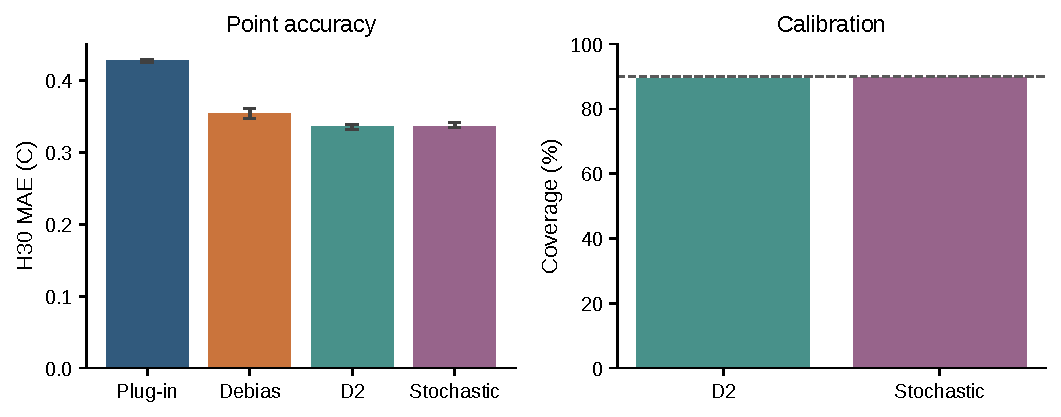
\includegraphics[width=\textwidth]{figures/simple_research/02_annual_comparators.pdf}\caption{Annual estimation under difficult controlled gaps. Both historical source-calibrated methods receive the same observed-bound projection and normal-spacing tail model. Bars show empirical repetition ranges within the same archive; these are not independent climates.}\label{fig:estimators}\end{figure}
\begin{figure}[p]\centering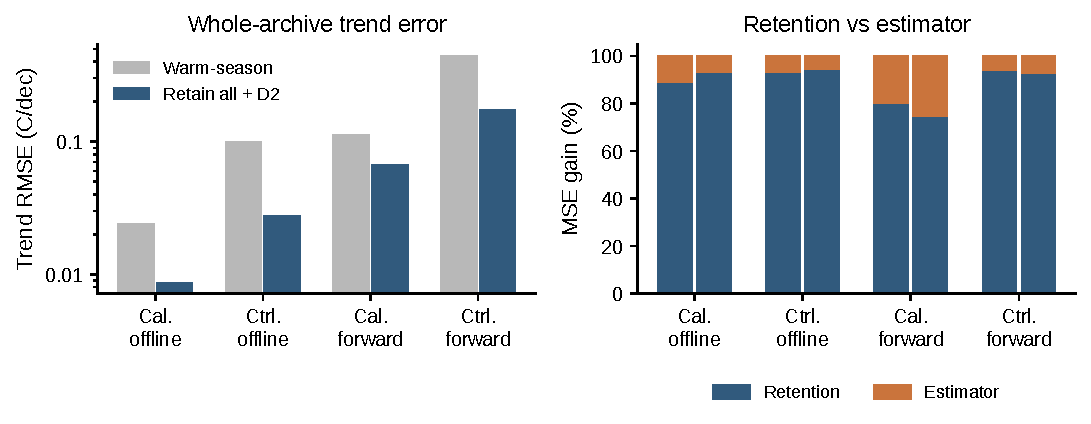
\includegraphics[width=\textwidth]{figures/simple_research/03_archive_factorial.pdf}\caption{Whole-archive trend errors and the symmetric retention/estimator decomposition. Left: D2 with identical masks and either retention set. Right: D2 and calibrated stochastic alternatives, with complete paired MSE cells. Contribution percentages are specific to each experimental setting.}\label{fig:whole-archive}\end{figure}
\begin{figure}[p]\centering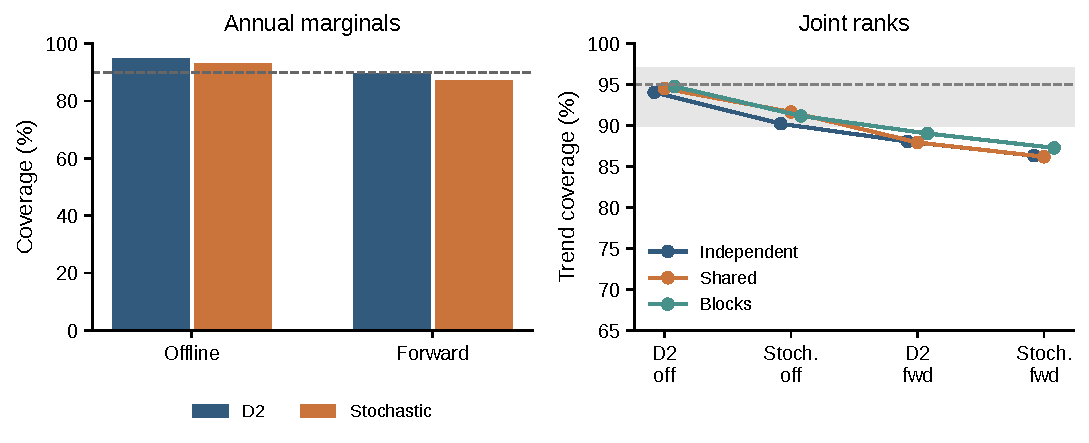
\includegraphics[width=\textwidth]{figures/simple_research/04_joint_uncertainty.pdf}\caption{Annual 90 percent and finite-record 95 percent trend intervals are evaluated separately. The rank methods preserve identical bounded annual marginals. Tail extrapolation is an assumption and source-group uncertainty is not shown by the bars.}\label{fig:joint-uncertainty}\end{figure}
\begin{figure}[p]\centering
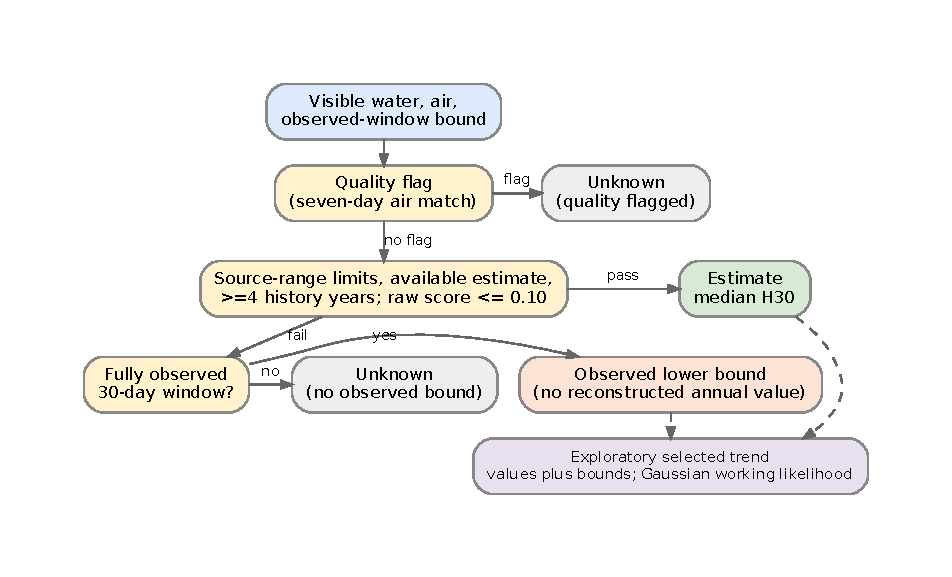
\includegraphics[width=\textwidth]{figures/architecture/fig2_release_actual.pdf}
\caption{The evaluated three-output decision and exploratory trend analysis. The cap applies to an individual raw classifier score, not a certified group risk. The seven-day water--air check was assessed only for the clean and imposed exact-air-substitution cases. The selected-trend working likelihood treats released values as exact and observed bounds as censored.}\label{fig:release-system}
\end{figure}
\begin{figure}[p]\centering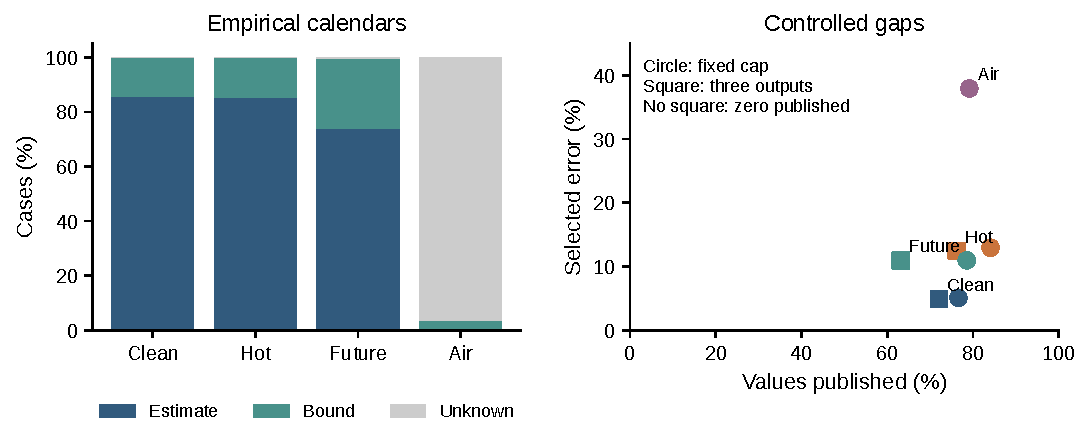
\includegraphics[width=\textwidth]{figures/simple_research/05_output_boundaries.pdf}\caption{Left: three outputs for empirical-calendar masks. Right: numerical-publication rates and selected errors for controlled gaps. Source diagnostics do not remove extrapolation failures. The air-agreement flag addresses the specified exact-substitution stress only; zero publication is shown as unknown rather than zero-risk success.}\label{fig:output-boundaries}\end{figure}

\bibliography{references_tr,references_review_completion}
\end{document}
